\documentclass{article}
\usepackage[a4paper]{geometry}
\usepackage[utf8]{inputenc}
\usepackage{polski}
\usepackage{tabularx}
\usepackage{indentfirst}
\usepackage{multirow}
\usepackage{amssymb}
\usepackage{amsmath}
\usepackage{anysize}
\usepackage{float}
\usepackage{caption}
\usepackage{subcaption}
\usepackage{graphicx}
\usepackage{tikz}
\usepackage{listings}
\usepackage{color}
\usepackage{verbatim}

\usetikzlibrary{shapes}

\definecolor{mygreen}{rgb}{0,0.6,0}
\definecolor{mygray}{rgb}{0.5,0.5,0.5}
\definecolor{mymauve}{rgb}{0.58,0,0.82}

\usepackage{titling}
\newcommand{\subtitle}[1]{%
	\posttitle{%
	\par\end{center}
	\begin{center}\small#1\end{center}
	\vskip0.5em}%
}

\title{Chariot}
\subtitle{Akademia Górniczo-Hutnicza im. Stanisława Staszica w Krakowie\\
	Wydział Elektrotechniki, Automatyki,\\
	Informatyki i Inżynierii Biomedycznej\\
	Informatyka, 3. rok, PWiR grupa 5a}
\author{Kacper Tonia\and
		Sławomir Kalandyk}
\date{22.01.2020}

\begin{document}
%------------------------------------------------------------
\maketitle

\section{Cel programu}
Zadaniem programu jest rozsyłanie wozów strażackich do~incydentów zgłaszanych za~pośrednictwem strony internetowej. Pula wozów jest ograniczona, zaś same pojazdy po~powrocie z~akcji przez pewien czas pozostają niedostępne (czas na~uzupełnienie zapasów, naprawy itd.).
\section{Moduły}
\begin{itemize}
	\item \textbf{main} -- uruchamia serwer i pełni rolę klienta.
	\item \textbf{central} -- reprezentuje centralę powiadamiania ratunkowego, której można zgłosić żądanie pomocy straży pożarnej. Moduł ten implementuje zachowanie \texttt{gen\_server}.
	\item \textbf{domain} -- definiuje rekord \texttt{state} używany przez serwer centrali, a~także tzw.~\emph{invoke functions} -- funkcje realizujące podstawową logikę aplikacji (zapisywanie zgłoszeń, wysyłanie wozów strażackich itd.).
	\item \textbf{firetrucks} -- definiuje rekord \texttt{firetruck} reprezentujący wóz strażacki, a~także podstawowe operacje z~tym rekordem związane.
	\item \textbf{server} -- serwer HTTP zaimplementowany za pomocą \texttt{httpd} zawierającego się w pakiecie \texttt{inets}; są~w~nim~definiowane funkcje odpowiadające na~zapytania GET/POST
\end{itemize}

\subsection{Serwer centrali}
Operacje realizowane przez serwer centrali możemy podzielić na~3~kategorie:
\begin{itemize}
	\item operacje opisane przez \texttt{handle\_call} są~synchroniczne, zwracają pewną wartość nie modyfikując stanu serwera.
	\begin{itemize}
		\item \texttt{get\_vehicles} pobiera aktualną listę pojazdów wraz z~ich stanem
	\end{itemize}

	\item operacje opisane przez \texttt{handle\_cast} są~asynchroniczne, nie blokują klienta. Nie zwracają istotnych wartości, ale mogą modyfikować stan serwera.
	\begin{itemize}
		\item \texttt{report\_incident} zgłasza incydent wymagający przyjazdu straży pożarnej
	\end{itemize}

	\item operacje opisane przez \texttt{handle\_info} sygnalizują serwerowi zajście jakiegoś zdarzenia. Nie powinny być wywoływane z~zewnątrz.
	\begin{itemize}
		\item \texttt{report\_enqueued} sygnalizuje, że~w~kolejce zgłoszeń znajdują się oczekujące zgłoszenia
		\item \texttt{dispatch\_finished} sygnalizuje, że~pojazd wrócił z~akcji strażackiej
		\item \texttt{preparation\_finished} sygnalizuje, że~pojazd jest gotowy do~następnej akcji strażackiej
	\end{itemize}
\end{itemize}

\begin{figure}[H]
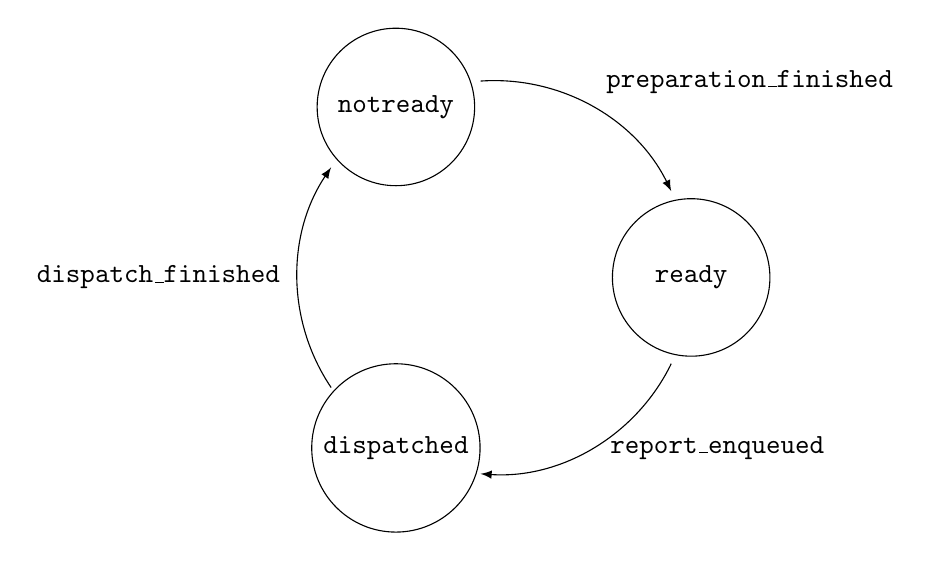
\begin{tikzpicture}[state/.style={circle, draw, minimum size=2cm}]

	\def \n {3}
	\def \radius {2.5cm}
	\def \margin {26} % margin in angles, depends on the radius
	
	\node[state] at (0:\radius) {\texttt{ready}};
	  \draw[<-, >=latex] ({0+\margin}:\radius)
		arc ({\margin}:{360/\n-\margin}:\radius);
	\node at (60:\radius) [above right=0.05cm] {\texttt{preparation\_finished}};
		
	\node[state] at ({ -360/\n }:\radius) {\texttt{dispatched}};
	  \draw[<-, >=latex] ({360/\n+\margin}:\radius)
		arc ({360/\n+\margin}:{360/\n * 2-\margin}:\radius);
	\node at (180:\radius) [left=0.1cm] {\texttt{dispatch\_finished}};
	
	\node[state] at ({ -360/\n * 2 }:\radius) {\texttt{notready}};
	  \draw[<-, >=latex] ({360/\n * 2+\margin}:\radius) 
		arc ({360/\n * 2+\margin}:{360/\n * 3-\margin}:\radius);
	\node at (300:\radius) [right=0.1cm] {\texttt{report\_enqueued}};
	
\end{tikzpicture}
\caption{Cykl pracy wozu strażackiego}
\end{figure}

\section{Główne komponenty programu i ich zadania}
\textbf{Main:}
\begin{enumerate}
	\item Tworzy pulę pojazdów
	\item Uruchamia serwer centrali
	\item Uruchomia serwer HTTP
\end{enumerate}

\textbf{Serwer centrali:}
\begin{enumerate}
	\item Zarządza pulą pojazdów
	\item Informuje serwer HTTP o stanie pojazdów
\end{enumerate}

\textbf{Serwer HTTP:}
\begin{enumerate}
	\item Po uruchomieniu, oczekuje na~zapytania GET/POST
	\item Przy zapytaniu GET: zwraca zserializowane pojazdy wraz z~ich obecnym stanem
	\item Przy zapytaniu POST: zleca zmianę stanu jednego z pojazdów na \texttt{dispatched}
\end{enumerate}

\textbf{Strona WWW:}
\begin{enumerate}
	\item Udostępnia pole tekstowe wraz z przyciskiem "Report incident", który po naciśnięciu wykonuje zapytanie POST
	\item Pokazuje obecne stany pojazdów w puli:
		\begin{itemize}
			\item \texttt{ready} -- barwa niebieska
			\item \texttt{dispatched} -- barwa pomarańczowa
			\item \texttt{notready} -- barwa żółta
		\end{itemize}
	\item Wyświetla logi - zserializowane rekordy pojazdów składające się z pól \texttt{id}, \texttt{status} oraz \texttt{waiting\_since}
	\item Co dany okres czasu (domyślnie 1s) odpytuje serwer o aktualny stan pojazdów
\end{enumerate}

\section{Diagramy sekwencji}
\begin{figure}[H]
	\includegraphics[width=.9\linewidth]{ChariotBase.png}
	\caption{Przebieg zapytania o stan pojazdów}
\end{figure}

\begin{figure}[H]
	\includegraphics[width=.9\linewidth]{ChariotCentral.png}
	\caption{Przebieg zgłaszania wypadku}
	
\end{figure}

\section{Pakiety zewnętrzne}
\begin{itemize}
	\item Jsone - pakiet służący nam do serializowania rekordów do formatu JSON, posiada licencję MIT
\end{itemize}

\section{Specyficzne rozwiązania}
\subsection{Problem "głodzenia" pojazdów}
Domyślnie pojazdem wysyłanym do wypadku byłby pojazd w stanie \texttt{ready} o najmniejszym identyfikatorze spośród takich pojazdów. Potencjalnie mogło to doprowadzić do sytuacji, gdy część pojazdów nigdy nie zostałaby wykorzystana. Przykładowo:
\begin{itemize}
	\item Posiadamy 6 pojazdów
	\item Pojazd 1 zmienia stan na \texttt{dispatched}, zaraz po nim przychodzi kolejna informacja o wypadku i pojazd 2 zmienia stan na \texttt{dispatched}
	\item Pojazd 1 wraca, zmienia stan na \texttt{notready} i zaraz później na \texttt{ready}
	\item Przychodzi informacja o wypadku: pojazd 1 zmienia stan na \texttt{dispatched}
\end{itemize}
Ostatecznie, gdyby taka sytuacja powtarzała się cały czas, pojazdy o ID 3, 4, 5, 6 potencjalnie mogłyby nie być w ogóle wykorzystywane.

Problem został rozwiązany poprzez dodanie do rekordu pojazdu parametru \texttt{waiting\_since}, który zapisuje czas, w którym pojazd ostatni raz zmienił stan na \texttt{ready}. Do wypadku wysyłany jest pojazd, który najdłużej nie był wykorzystywany - różnica pomiędzy czasem obecnym, a zapisanym jest największa spośród pojazdów.

\section{Instrukcja obsługi}
\begin{enumerate}
	\item W katalogu projektu wywołaj "make compile"
	\item Wykonaj "cd beam", a potem "escript main.beam" (przejście do katalogu beam i uruchomienie programu)
	\item Wejdź w przeglądarce internetowej na adres localhost:8080
\end{enumerate}

\section{Ograniczenia programu}
\begin{itemize}
	\item Liczba wozów strażackich jest określona przy starcie programu, nie można jej zmienić po starcie programu
	\item Pojazdy straży nie są w jakikolwiek sposób rozróżnialne od siebie
	\item Akcje, na które wysyłane są wozy strażackie są imitowane funkcją \texttt{timer:sleep()}. W stanie \texttt{dispatched} pojazd przebywa od 5 do 15 sekund, a w stanie \texttt{notready} od 2 do 12 sekund
\end{itemize}

\section{Możliwe rozszerzenia programu}
Jednym z możliwych rozszerzeń jest dodanie różnych typów wypadków i możliwość wyboru wypadku. Nadałoby to sens rozróżnieniu pojazdów ze względu na wyposażenie - to, czy pojazd mógłby wyruszyć do akcji zależałoby od tego, czy jest odpowiednio wyposażony, aby móc efektywnie nieść pomoc na miejscu zdarzenia.
\end{document}